\documentclass[
  % all of the below options are optional and can be left out
  % course name (default: 2IL50 Data Structures)
  course = {{MATH102 Calculus II}},
  % quartile (default: 3)
  quartile = {{2}},
  % assignment number/name (default: 1)
  assignment = 2,
  % student name (default: Some One)
  %name = {{Some One ; Other Person}},
  % student number, NOT S-number (default: 0123456)
  %studentnumber = {{0123456 ; 0314159}},
  % student email (default: s.one@student.tue.nl)
  %email = {{s.one@student.tue.nl ; o.person@student.tue.nl}},
  % first exercise number (default: 1)
  firstexercise = 1,
  term = 202
]{aga-homework}
\usepackage{graphicx}
\usepackage{advdate}
\usepackage{amsmath}
\usepackage[shortlabels]{enumitem}


\begin{document}
%\noindent {\hfill \vspace{-2\baselineskip} {\footnotesize\bf  Due \AdvanceDate[14]\today  \; midnight} \vspace{3mm}}

\begin{center}
  {\large
  \begin{tabular}{|l|l|}
    \hline
    % after \\: \hline or \cline{col1-col2} \cline{col3-col4} ...
    Group Number: & \hspace{3in} \\
     &  \\ \hline
    Members: &  \\
        &  \\ \cline{2-2}
        &  \\
        &  \\ \cline{2-2}
        &  \\
        &  \\ \cline{2-2}
        &  \\
        &  \\ \cline{2-2}
        &  \\
        &  \\ \cline{2-2}
        &  \\
        &  \\ \cline{2-2}
        &  \\
        &  \\ \cline{2-2}
        &  \\
        &  \\ \cline{2-2}
        &  \\
        &  \\ \cline{2-2}
        &  \\
        &  \\ \cline{2-2}
        &  \\
        &  \\ \cline{2-2}
        &  \\
        &  \\ \cline{2-2}
        &  \\
        &  \\ \cline{2-2}
        &  \\
        &  \\ \cline{2-2}
        &  \\
        &  \\ \cline{2-2}
        &  \\
        &  \\
    \hline
  \end{tabular}
  }
\end{center}


\newpage

\problem  If $R_n$ is the Riemann sum for $f(x)= 4 + \frac{x^2}{8}, 0 \leq x \leq 4$
with $n$ subintervals and taking sample points to be the right end points, then $R_n =$


\newpage

\problem $\lim_{n\to \infty}\sum_{i=1}^n\frac{1}{n}\cos\left(1+\frac{i}{n}\right)^2=$

\begin{enumerate}[(A)]
  \item $\int_{1}^{2}\cos(1+x^2)dx$.
  \item $\int_{1}^{2}\cos(x^2)dx$.
  \item $\int_{1}^{2}\cos^2(x)dx$.
  \item $\int_{0}^{1}\cos(x^2)dx$.
  \item $\int_{0}^{1}\cos(1+x^2)dx$.
\end{enumerate}

\newpage


\problem
\begin{minipage}[t]{0.6\textwidth}
\vspace{0pt}
  In the figure shown, regions $A$ and $B$ are bounded by the graph of a function $f$ and the $x$-axis. If the area of region $A$ is $\frac{1}{6}$ and the area of the region $B$ is $\frac{3}{8}$, then
  \[
  \int_0^4f(x) dx + \int_{0}^{4}|f(x)| dx =
  \]
\end{minipage}
\begin{minipage}[r]{0.4\textwidth}
	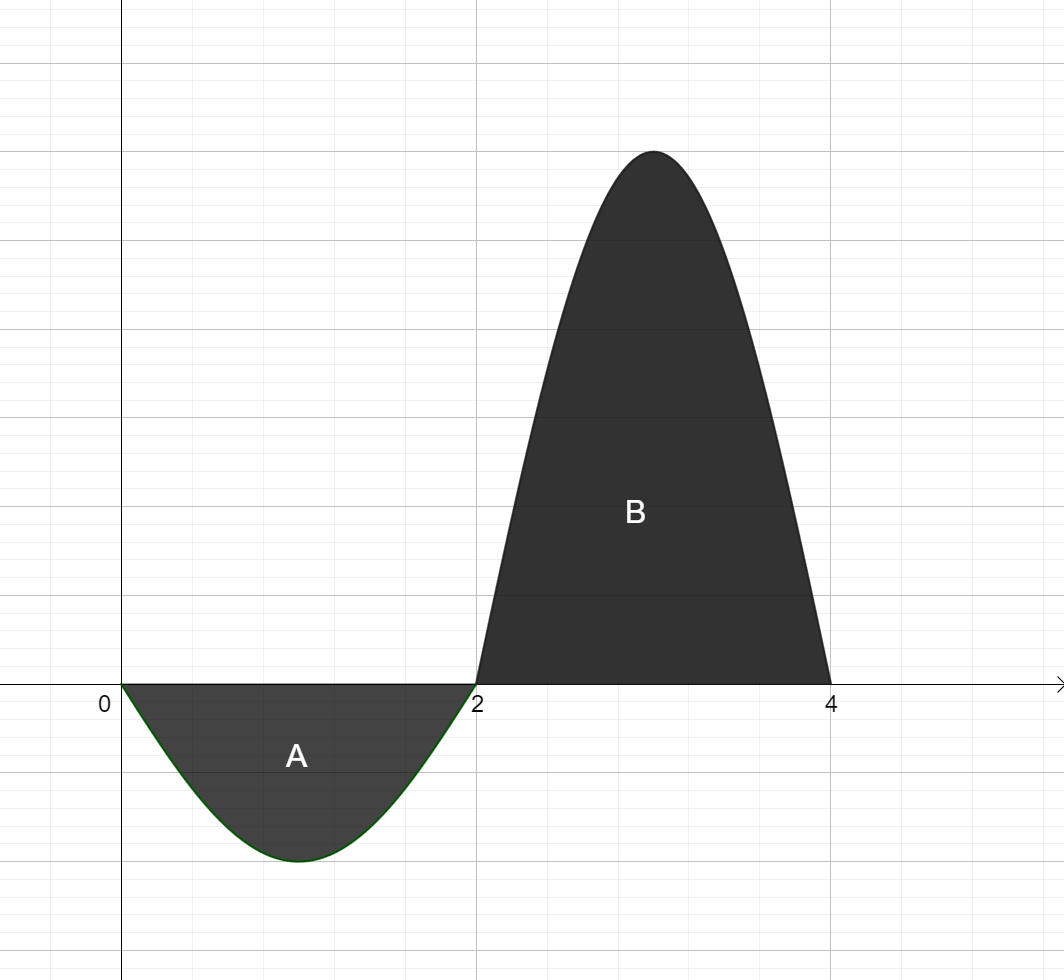
\includegraphics[width=\textwidth]{figures/ps2fig1.png}
\end{minipage}



\end{document} 